\chapter{软硬件补偿方法的性能对比}
在第4章和第5章分别介绍了干涉仪环境误差补偿在软件层面的解决方法和硬件层面的加速补偿方法,任何一者都可以实现基于粒子群算法的对双频激光干涉仪环境误差的补偿,但两者各有优劣,软件层面的基于温度梯度的分段式粒子群算法补偿效果能够较好地适用于各种场景下的环境误差补偿,并且补偿方法简单,只需要增加额外的温度传感器和气压传感器,但在\ref{基于温度梯度的分段粒子群算法补偿方法的不足之处}节中说明了该方法对运行时间有着较大的要求;而硬件层面的加速补偿方法,由于设计专用的并行加速模块,使得运行速度能得到一定提升,但是由于算法硬化过程中产生的截断误差、适应度模型改变等原因,使得其精度稍有降低,并且补偿方法较为复杂,不仅需要增加气压传感器和温度传感器,还需要增加专门的定制电路或FPGA开发板,而且在寄存器配置等软硬协同操作上复杂一些。所以两种方法各有优劣,本章将会详细对比一下两种方法的优缺之处,为了比较结果更加明显,若无特别强调,以下均是整段式粒子群算法,种群数量均为32,迭代次数均为100次。
\section{运行时间对比}
运行时间是最关心的性能参数之一,它的快慢直接影响了补偿的性能与补偿的实时性。使用图\ref{fig:短时测量实验数据}所示数据在matlab中进行粒子群算法的运行时间分析,结果如图\ref{fig:软件运行时间结果图}所示。处理后的样本长度约为382个点,迭代次数为100,所需迭代时间约为0.499秒。软件层面的运行时间与CPU性能息息相关,实验用电脑的CPU为AMD 的R7-6800H,8核16线程,主频为3.2GHz,多核睿频可达4.0GHz,单核睿频可达4.7GHz,TDP热功耗为45W。
\begin{figure}[htb]
  \centering
  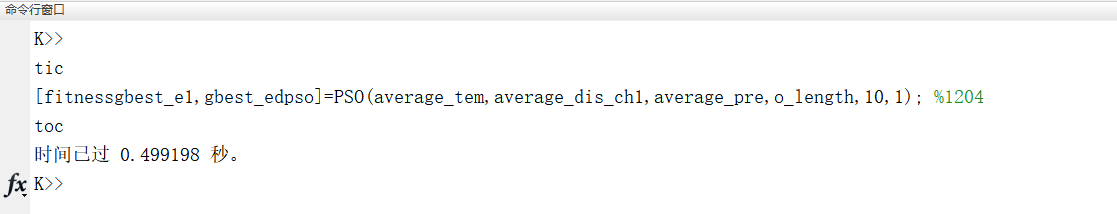
\includegraphics[width=14cm]{fig/6-fig/软件运行时间.png}
  \caption{软件运行时间结果图}
  \label{fig:软件运行时间结果图}
\end{figure}

而硬件的运行时间取决于计算周期数和时钟周期大小,运算周期数由设计决定,同样的计算量运算周期数一般是固定的,而时钟周期大小由设计的时序路径以及时序约束决定。本文所列的时序约束主要包含时钟约束、输入约束和输出约束等。时钟约束主要为设定主时钟,主时钟通常通过输入端口引入,指定周期以及可选的名称和波形(上升沿和下降沿时间),并描述占空比,设定的时钟周期为20ns,占空比为50$\%$。输入延迟描述FPGA边界处的输入信号与时钟(通常是板时钟)之间的相对相位,如图\ref{fig:输入延迟示意图}所示,主要由tco和trce$\_$dly两项组成,tco是来自输入FPGA芯片的延迟,需要查阅FPGA手册得出,trec$\_$dly是来自PCB板的延迟,一般难以得到准确值。输出延迟描述参考时钟与FPGA边界处的输出信号之间的相对相位,由tsu、thd和trce$\_$dly三项组成,tsu和thd分别为建立时间和保持时间,需要查阅FPGA手册得到。
\begin{figure}[htb]
  \centering
  \subfigure[输入延迟示意图]{
    \begin{minipage}[b]{0.90\textwidth}
      \centering
      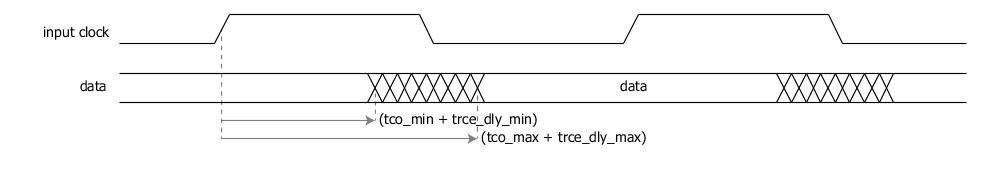
\includegraphics[width=12cm]{fig/6-fig/输入延迟示意图.png}
    \end{minipage}
    \label{fig:输入延迟示意图}
  }
  \subfigure[输出延迟示意图]{
    \begin{minipage}[b]{0.90\textwidth}
      \centering
      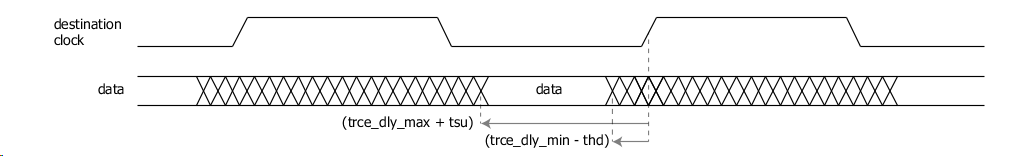
\includegraphics[width=12cm]{fig/6-fig/输出延迟示意图.png}
    \end{minipage}
    \label{fig:输出延迟示意图}
  }
  \caption{输入输出延迟示意图}
  \label{fig:输入输出延迟示意图}
\end{figure}

以下是三种时序约束的部分示例:
\begin{enumerate}
  \item 时钟约束:create$\_$clock -period 20.000 -name i$\_$clk -waveform {0.000 10.000} [get$\_$ports i$\_$clk]
  \item 输入延迟约束:set$\_$input$\_$delay -clock [get$\_$clocks i$\_$clk] -min -add$\_$delay 5.0 [get$\_$ports {i$\_$pfc$\_$in$\_$last$\_$v[0][*]}]
  \item 输出延迟约束:set$\_$output$\_$delay -clock [get$\_$clocks i$\_$clk] -min -add$\_$delay 4.0 [get$\_$ports {o$\_$pfc$\_$out$\_$fitness[*]}]
\end{enumerate}

时序检查的结果如图\ref{fig:时序检查结果图},在设定检查频率为50MHz时最差的时序裕量还有5.844ns,理论上可以跑通更高的时钟频率,但是为了可靠性考虑,留足了足够的时序裕量,最终粒子群算法加速补偿系统的时钟频率为50MHz。
\begin{figure}[htb]
  \centering
  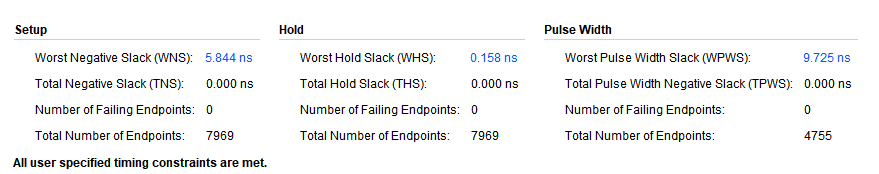
\includegraphics[width=14cm,height=3.5cm]{fig/6-fig/时序检查结果.png}
  \caption{时序检查结果图}
  \label{fig:时序检查结果图}
\end{figure}

使用图\ref{fig:短时测量实验数据}所示数据在vivado中进行粒子群算法的加速时间分析,结果如图\ref{fig:硬件运行时间结果图}所示。处理后的样本长度约为382个点,最大迭代次数为100,从图中可以看出前4000ns为软件配置寄存器的时间,第4200ns时start信号拉高,代表寄存器配置信息已经生成,可以开始对粒子群加速补偿系统进行配置,同时busy信号也拉高了,代表系统开始工作,在约7000ns时done信号产生脉冲,代表该次粒子群算法训练结束。
\begin{figure}[htb]
  \centering
  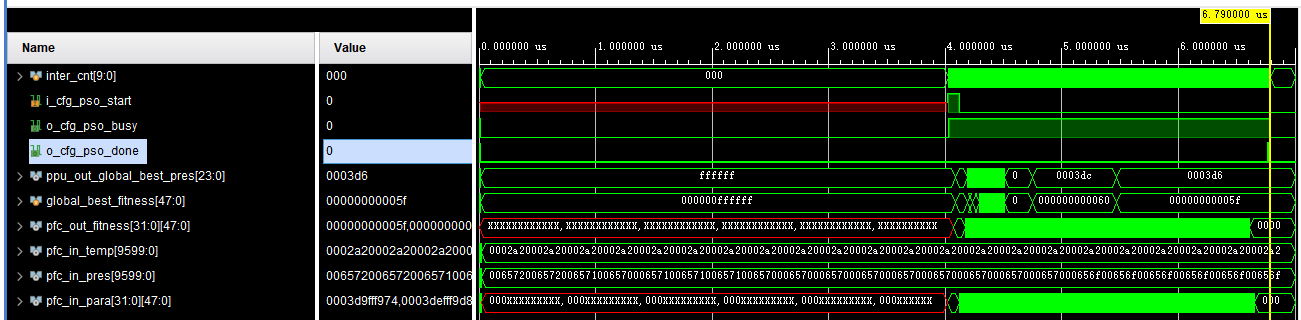
\includegraphics[width=14cm,height=5cm]{fig/6-fig/硬件运行时间.png}
  \caption{硬件运行时间结果图}
  \label{fig:硬件运行时间结果图}
\end{figure}

但软硬和硬件的运行时间都是和所设置的种群个体数强相关的,如图\ref{fig:运行时间和种群大小的关系图}所示,展示了种群大小在16-96之间,软件和硬件的运行时间关系,其中蓝色曲线代表的是软件运行时间,随着种群大小的增大而不断增大;而绿色曲线是硬件运行时间,由于硬件并行设置的加速单元只有32个,所以硬件计算时间是每当种群大小增大32时翻一倍(寄存器配置时间的增长在此处忽略不计),因为种群大小每增加32,在计算一次迭代时需要多运算一个周期。
\begin{figure}[htb]
  \centering
  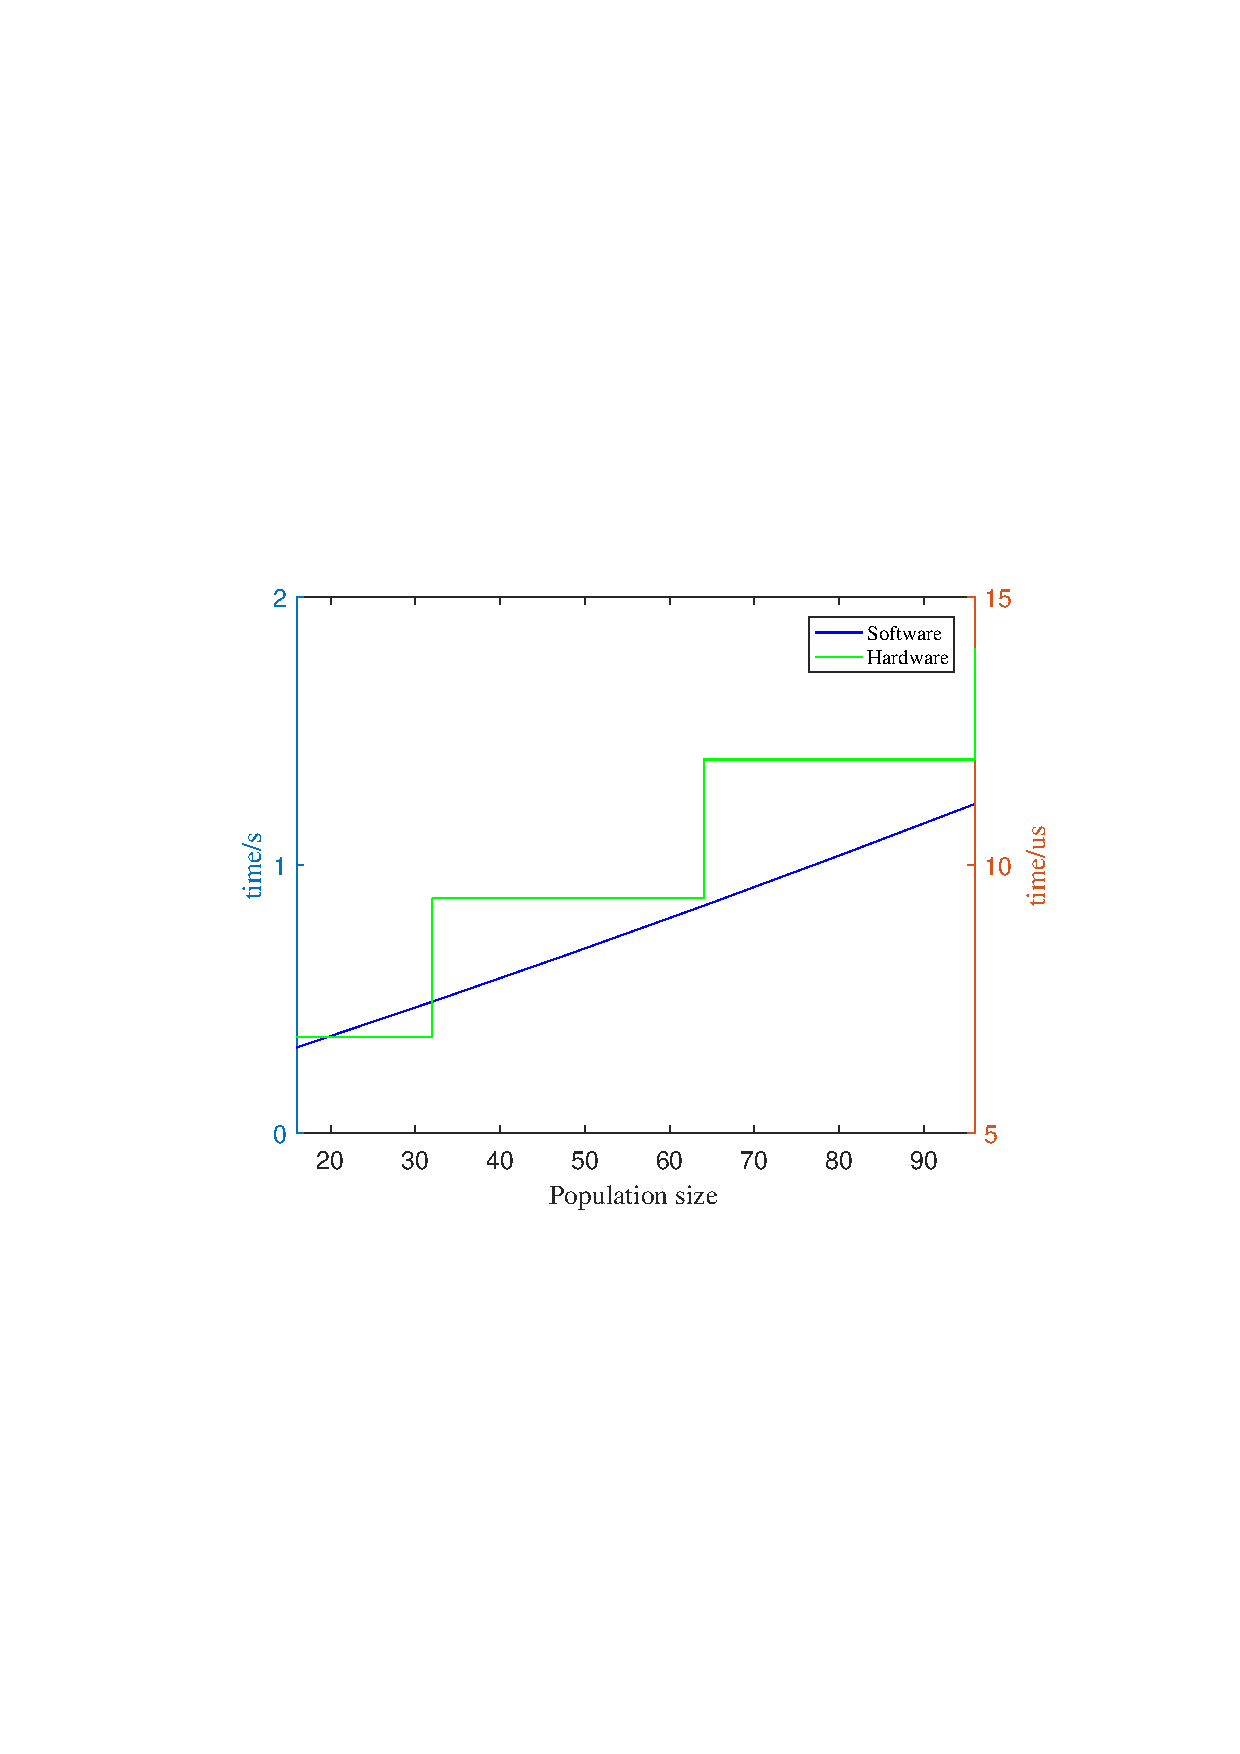
\includegraphics[width=10cm]{fig/6-fig/运行时间和种群大小的关系.pdf}
  \caption{运行时间和种群大小的关系图}
  \label{fig:运行时间和种群大小的关系图}
\end{figure}

\section{所需资源对比}
采用软件方法进行补偿,所有计算均在CPU上进行,无需任何其他辅助计算模块,而采用硬件方法进行补偿则需要使用大量的FPGA资源,如表\ref{tab:资源使用表}所示,主要使用的资源为LUT、FF和DSP,LUT为查找表(Look-Up-Table),常用于大部分的组合逻辑,FF为触发器(Flip Flop),用于时序逻辑中存储数据,DSP为数字信号处理器(Digital Signal Processing),用于各模块中的乘法逻辑。
\begin{table}[H]
  \centering
  \caption{资源使用表}
  \label{tab:资源使用表}
  \begin{tabular}{c|c|c|c}
      \hline
                                    & LUT        & FF        &DSP            \\ \hline
      pso$\_$fitness$\_$cal         & 12761      & 4775      & 210           \\ \hline
      pso$\_$population$\_$upda     & 2389       & 5449      & 0              \\ \hline
      pso$\_$velocity$\_$cal        & 397        & 193       & 15             \\ \hline
  \end{tabular}
\end{table}

需要特别强调的是,pso$\_$fitness$\_$cal模块和pso$\_$velocity$\_$cal模块是和种群的个体数强相关的,所以在预估资源消耗时需要进行乘法,而pso$\_$population$\_$upda模块则是弱相关,即使种群个体数改变也只需在表格数据的基础上进行轻微增加即可。资源瓶颈为DSP数量,所以在设定种群个体数IND$\_$NUM这一parameter时需要先进行资源评估。

\section{补偿效果对比}
图\ref{fig:软硬件补偿效果对比图}为软硬件补偿效果的对比图,所使用的数据为图\ref{fig:短时测量实验数据}。(a)图为测量臂长度为45mm的位移测量数据,(b)图为测量臂长度为45mm的位移测量数据,(c)图为对应的温度和气压数据,(a)、(b)、(c)三图的横轴均为时间,单位为h;(a)和(b)图中的竖轴为位移数据,单位为nm,带方块标注的紫色曲线为经上文设计的粒子群算法加速补偿系统硬件补偿之后的位移数据,带红色菱形标注的为使用粒子群算法优化后的软件补偿后位移数据,(c)图的竖轴为温度和气压数据,单位为$^{\circ} \mathrm{C}$和kPa,其中带圆圈标注的蓝色曲线为温度数据,红色曲线为气压数据。

\begin{figure}[htb]
  \centering
  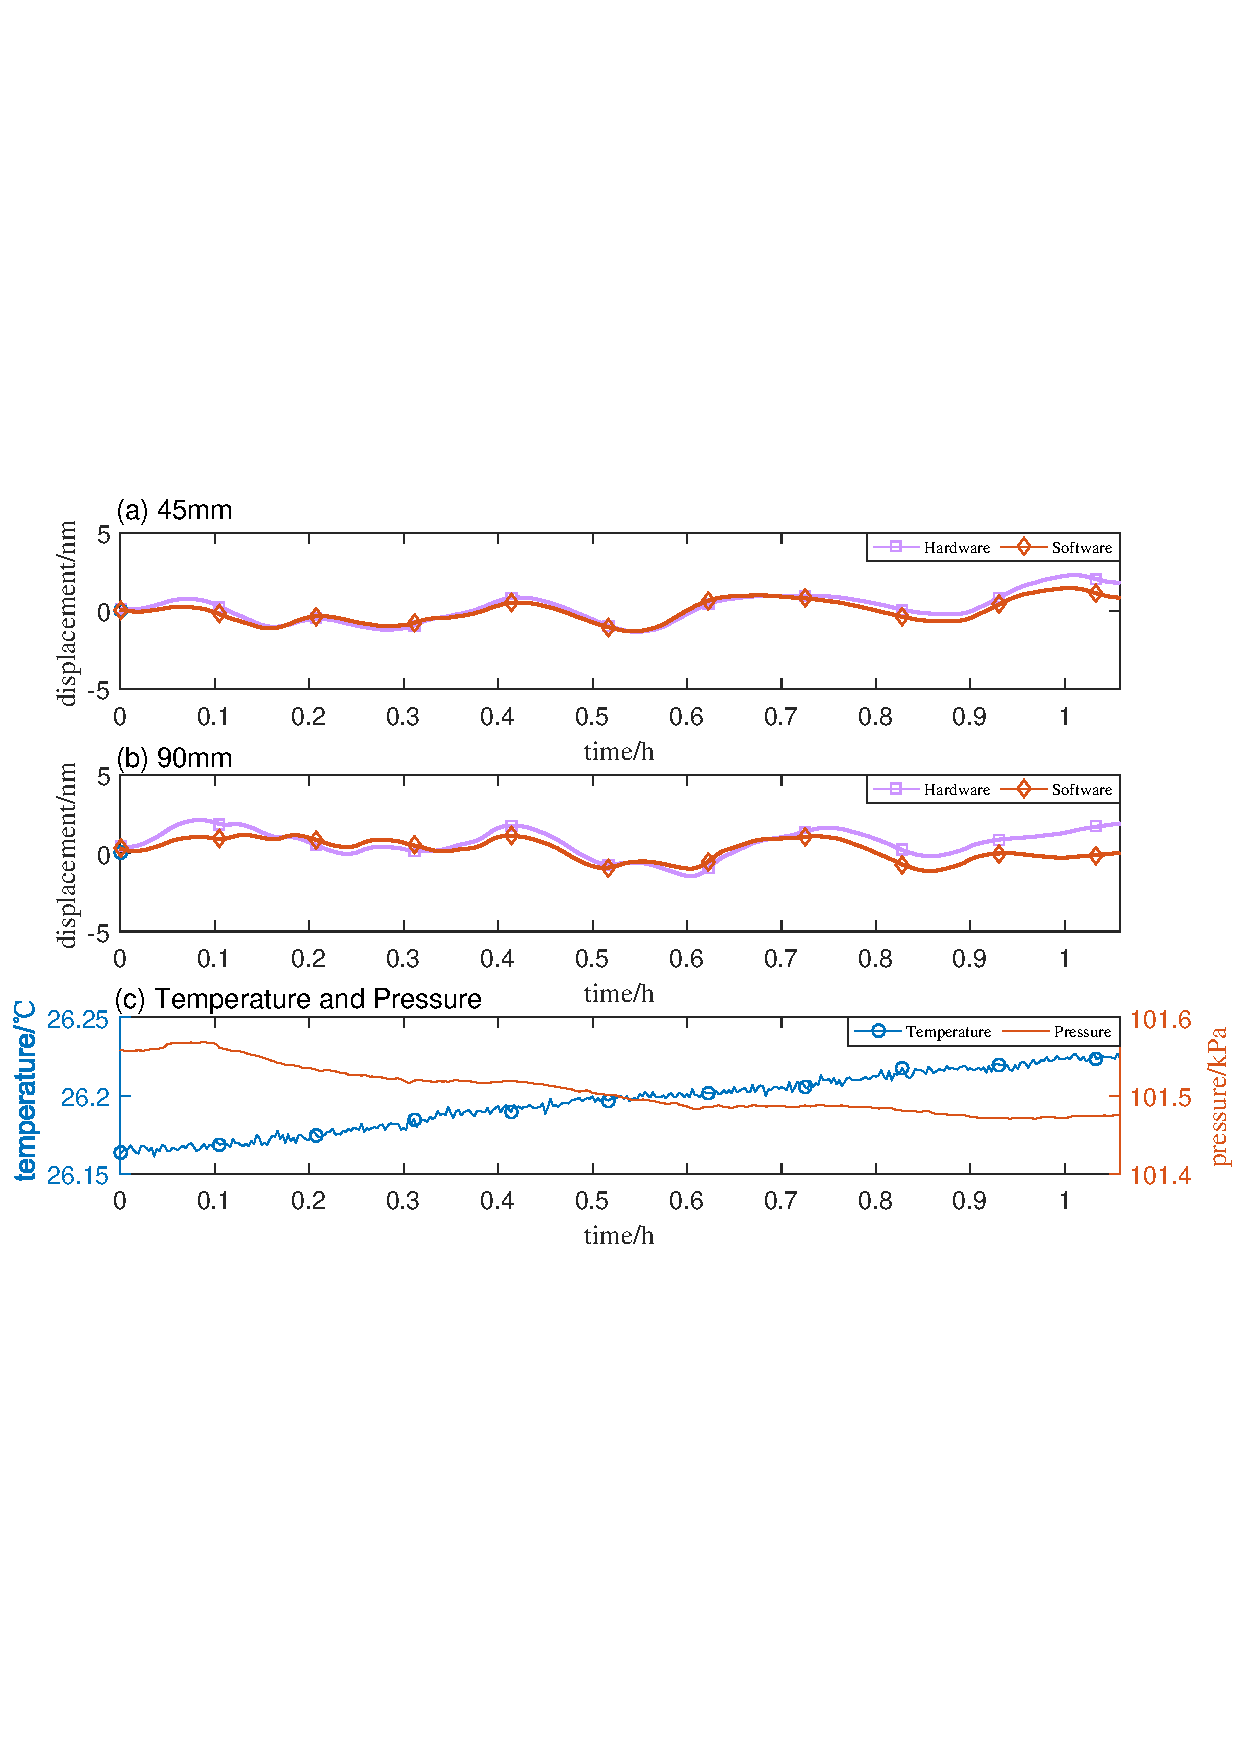
\includegraphics[width=14cm]{fig/6-fig/软硬件补偿效果对比.pdf}
  \caption{软硬件补偿效果对比图}
  \label{fig:软硬件补偿效果对比图}
\end{figure}
如图\ref{fig:软硬件补偿效果对比图}所示,代表硬件补偿效果的紫色曲线和软件补偿效果的黄色曲线都十分接近零点,这说明两者在对环境误差的补偿上较图\ref{fig:短时测量实验数据}都取得了更好的补偿效果,并且两条曲线相隔的最大距离为0.9nm,这说明两种方法的补偿效果十分接近。红色曲线在测量臂长度为45mm和90mm的两组数据下,补偿后的残留均方根误差只有0.8541nm和1.034nm,而紫色曲线在测量臂长度为45mm和45mm的两组数据下,补偿后的残留均方根误差只有0.8225nm和1.112nm,最大误差约为7.5$\%$。需要特别说明的是,这个误差百分比最高可以达到约8$\%$,但较大的误差百分比只会在数值本身很小的情况下出现,所以绝对误差值很小,总体而言误差处在一个可以接受的范围内。

并且可以看出在测量臂长度为45mm的数据组中,硬件补偿后的效果较软件补偿更好,这是由于虽然硬件补偿有截断误差,但是由于粒子群算法本身就有较大的随机性,这一点从式\eqref{eq:粒子群算法速度更新}中两个随机数就可以看出,所以截断误差可能在某些情况下会加剧粒子群算法的随机情况从而造成较好的补偿效果,但在大多数情况下,截断误差只会导致补偿效果变差。

\section{优缺点总结}
干涉仪环境误差补偿软件层面的解决方法和硬件层面的加速补偿方法,任何一者都可以实现基于粒子群算法的对双频激光干涉仪环境误差的补偿,但两者各有优劣。总体而言软件层面在资源、补偿效果和复杂程度等方面占有优势,而硬件加速补偿由于截断误差、设计方法较为复杂等原因在这些方面处于劣势,但是由于硬件上并行设置了大量的加速单元,所以使得硬件加速补偿方法在运行时间上占有较大优势,所以比较适用于对补偿速度要求较高的场合或者用于前文提出的基于温度梯度分段补偿方法中的加速场合,而软件补偿方法由于其简便性和良好的补偿效果,适用于大部分的补偿场景,如表\ref{tab:软硬件优缺点总结表}所示。
\begin{table}[H]
  \centering
  \caption{软硬件优缺点总结表}
  \label{tab:软硬件优缺点总结表}
  \begin{tabular}{c|c|c}
      \hline
                                    & 软件直接补偿        & 硬件加速补偿                  \\ \hline
      运行时间                       & 毫秒级             & 微秒级                        \\ \hline
      电路资源                       & 无需外加其他电路    & 需外加电路,DSP资源紧张        \\ \hline
      补偿效果                       & 较好               & 差一些,不超过8$\%$的误差     \\ \hline
      复杂程度                       & 低                 & 较高                          \\ \hline
      适用场合                       & 适用于大部分场合    & 适用于高速场合或用于分段式补偿的加速场合 \\ \hline
  \end{tabular}
\end{table}

\section{本章小结}
本章主要介绍了干涉仪环境误差补偿软件层面的解决方法和硬件层面的加速补偿方法的优缺点,首先在运行时间方面介绍了软件补偿使用的CPU及运行时间,硬件加速补偿所下的时序约束及运行,并且介绍了两者运行时间随着种群大小的变化曲线。随后介绍了两种方法所消耗的资源以及补偿效果,通过数据分析硬件加速补偿的误差处在一个可接受的范围之内。最后对两种方法的优缺点及适用场合进行了一个总结。